
Laskuvarjot ja niiden suorituskyky kehittyvät jatkuvasti. Oppilasvarjot on kuitenkin kautta aikojen suunniteltu käyttövarmoiksi ja virheitä anteeksiantaviksi lentolaitteiksi. 1970-luvulla oppilaat hyppäsivät alkeispallovarjoilla. 1980-luvulla oppilaat käyttivät tehovarjoja ja kokeneemmat hyppääjät liitovarjoja. 1990-luvun alussa oppilasvarjoissa siirryttiin F-111-kankaisiin sekä suuriin, korkeaprofiilisiin varjoihin kuten Manta ja Raider. 1990-luvun lopulla ja 2000-luvun alussa alettiin käyttää ZP-kankaisia, lievästi elliptisiä oppilasvarjoja (esim. Navigator, Skymaster). Ne ovat kevyempiä ohjata ja säilyttävät lento-ominaisuutensa pidempään kuin edeltäjänsä. 


Kelpoisuushyppääjien käyttämät varjot ovat vuosien kuluessa kehittyneet nopeammin kuin oppilasvarjot. Käytetyt siipikuormat ovat kasvaneet ja varjomallit kehittyneet jatkuvasti. Monelle jo siirtymä oppilasvarjosta omaan varjoon voi olla melko suuri. On hyvä muistaa, että suuremmalla siipikuormalla lentäminen vaatii paljon keskittymistä turvallisen lentämisen opetteluun.  


Hyppääjän on osattava valita varjonsa ominaisuudet omien kykyjensä, harrastamansa lajin ja hyppy-ympäristönsä mukaan. Varjolla lentämisen tulee olla mukavaa ja turvallista sekä itselle että muille ilmassa oleville. Lisäksi hyppääjän tulee olla ymmärtää oman varjonsa ominaisuudet erilaisissa tilanteissa. Siksi onkin tärkeää tutustua tämän oppaan osaan Kuvunkäsittelyopas, kun siirrytään oppilaskalustosta nopeampiin varjoihin. 

\section{ Laskuvarjoja koskevat kokemusrajat }
\label{omiin-varusteisiin-siirtyminen-laskuvarjoja-koskevat-kokemusrajat}


Jatkokoulutuksessa oleva oppilas voi saada koulutuspäälliköltä tai apulaiskoulutuspäälliköltä luvan käyttää omia varusteitaan ja laskuvarjoaan. SIL ylläpitää luetteloja, joista ilmenee, mitkä varjomallit ovat soveltuvia 

\begin{itemize}
\item  alkeis- ja peruskoulutuksessa oppilaiden käyttöön 
\item  jatkokoulutuksessa oppilaiden käyttöön (koulutuspäällikön/apulaiskoulutuspäällikön suostumuksella)  
\item  itsenäisillä lisenssihyppääjillä  
\end{itemize}

SIL on määritellyt hyppääjille siipikuormarajat (katso siipikuorman määrittely) kokemuksen mukaan seuraavasti: 

\begin{itemize}
\item  alkeis- ja peruskoulutusvaihe < 1,1 lbs/ft². 
\item  jatkokoulutusvaihe sekä A- ja B-lisenssit < 1,34 lbs/ft². 
\end{itemize}

Koulutus- ja turvallisuuskomitea suosittelee jatkokoulutusvaiheen oppilaille ja ensimmäistä varjoaan hankkiville hyppääjille korkeintaan 1,1 siipikuormaa. 


Kelpoisuushyppääjien käytössä olevien varjojen erot oppilasvarjoihin ovat seuraavia: 

\begin{itemize}
\item  pienempiä, suurempi siipikuorma ⇒ suurempi nopeus alas- ja eteenpäin, kasvanut vajaatoimintaherkkyys, suurempi sakkausnopeus ⇒ vaativat suurempaa tarkkuutta ja reaktionopeutta 
\item  siipiprofiililtaan ja muodoltaan suorituskykyisempiä ⇒ parempi liitosuhde, suurempi nopeus ja käännösherkkyys 
\item  ohuet microline-punokset ⇒ välittävät avausnykäyksen voimakkaammin, kuluvat nopeammin, vaaralliset törmättäessä varjon varassa 
\item  lisävarusteet (tukahdutettava slider ja tukahtuva apuvarjo) vaativat huolellisuutta pakkaamisessa ja lentämisessä. 
\end{itemize}

\begin{figure*}[]\centering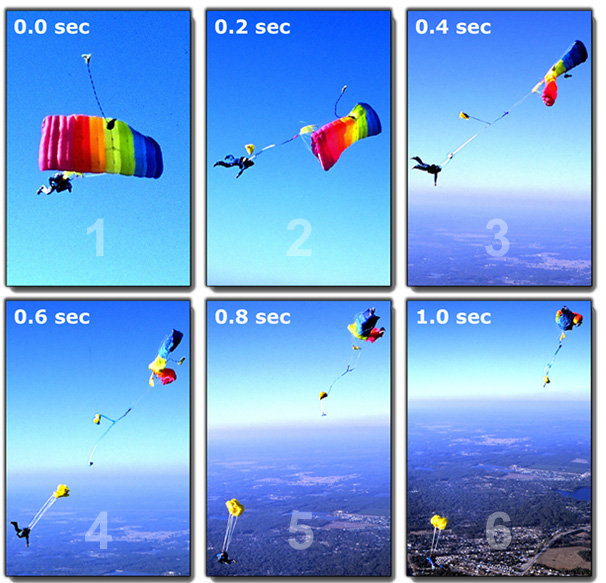
\includegraphics[width=0.7\textwidth]{MARD.jpg}\caption{MARD-järjestelmä voi nopeuttaa varavarjon avautumista. (kuva: UPT)}\end{figure*} 

\section{ Muut varusteet }
\label{omiin-varusteisiin-siirtyminen-muut-varusteet}


AAD (Automatic Activation Device) eli varavarjon automaattilaukaisin on oppilasvarjoissa sekä A- ja B-lisenssin hyppääjillä pakollinen varuste ja on nykyään vakiovaruste lähes kaikissa uusissa Suomeen tilattavissa varjopaketeissa. AAD:n käyttö kaikessa hyppäämisessä on erittäin suositeltavaa.  


Uusimmilla ja nopeimmilla varjoilla on hetkellisesti saavutettu pystynopeuksia, jotka ylittävät AAD:n virittymiskynnyksen (esimerkiksi expert-Cypresilla 35 m/s). AAD:n aktivoituminen vauhditetussa laskeutumisessa ei kuitenkaan ole mahdollista kuin suurilla siipikuormilla. AAD on pelastanut maailmalla jo satoja hyppääjiä. SIL on luetteloinut Suomessa käyttöön soveltuvat automaattilaukaisimet. 


RSL (Reserve Static Line) tarkoittaa varavarjon pakkolaukaisuhihnaa. Sen tarkoituksena on varmistaa varavarjon avautuminen päävarjon irrottua valjaista. Järjestelmä liittää päävarjon kantohihnan ja varavarjon aukaisujärjestelmän yhteen. RSL on hyvä apuväline, joka voi pelastaa hengen esimerkiksi matalan päävarjon irtipäästön jälkeen. Oppilasvarjoissa sekä A- ja B-lisenssihyppääjille RSL on pakollinen varuste. 


RSL-järjestelmään on saatavissa myös MARD-modifikaatio (Main assisted reserve deployment). MARD-järjestelmässä irti päästetty päävarjo avustaa varavarjon avautumista. Tämä nopeuttaa varavarjon avautumista ratkaisevasti. Tilanteissa, joissa irti päästetty päävarjo ei pysty nopeuttamaan varavarjon avautumista, RSL toimii normaalisti. MARD-järjestelmät ovat valmistajakohtaisia (esim. DRD, Reserve boost ja Skyhook), eikä niitä välttämättä ole saatavilla kaikkiin valjaisiin. RSL:n hihnan tulee olla kytkettynä, jotta MARD voi toimia. 


Kypärän/suojapäähineen käyttö on pakollista D-lisenssiin asti. Myös D-lisenssihyppääjät käyttävät yleensä hypätessään kovaa kypärää. Jos myöhemmin A-lisenssin saatuasi alat harjoitella nopeita laskeutumisia, käytä aina kovaa kypärää. 


Sopivan kypärän valintaan vaikuttaa esimerkiksi hyppylaji. Avokypärä mahdollistaa hieman laajemman näkökentän, mutta integraalikypärä suojaa mahdollisessa törmäyksessä myös hyppääjän leukaa ja kasvoja. Integraalikypärää käyttäessä kannattaa huomioida, että suljettu visiiri voi välillä huurtua. Visiirin avaamista ja sulkemista on syytä harjoitella etukäteen. Esimerkiksi tavallista paksummat käsineet voivat vaikeuttaa visiirin avaamista kuvun varassa.   


Useimmat hyppääjät käyttävät käsikorkeusmittaria. Mittarin voi sijoittaa kuitenkin myös muualle kuin ranteeseen. Analogisen korkeusmittarin voi esimerkiksi kiinnittää rintahihnaan. Digitaalista, numeronäyttöistä mittaria voi puolestaan käyttää reiteen tai käsivarteen kiinnitettynä. Tärkeintä mittarin käytössä on se, että käytetään aina samassa paikassa olevaa mittaria ja opetellaan lukemaan visuaalista mittaria kaikissa lentoasennoissa sekä kuvun varassa.  


Monet hyppääjät käyttävät visuaalisen mittarin lisäksi äänikorkeusmittaria. Niissä on usein 2–3 säädettävää hälytysrajaa, jotka hyppääjä voi asettaa haluamiinsa korkeuksiin. Äänikorkeusmittarit voivat myös tallentaa tietoa esimerkiksi hyppykorkeudesta, vapaapudotusajasta ja -nopeudesta sekä avauskorkeudesta. 


Äänikorkeusmittarit ovat hyvin luotettavia ja ne ovat hyödyllisiä lisävarusteita lähes kaikessa hyppäämisessä. Eritoten freehyppäämisessä, kameran tai muun lisälaitteen kanssa hypätessä äänikorkeusmittari on liki pakollinen varuste.  Äänikorkeusmittari on kuitenkin vain varmistusväline, korkeutta on jokaisella hypyllä tarkkailtava myös visuaalisesta mittarista.  


Korkeusmittarit ovat kaiken kaikkiaan hyvin luotettavia laitteita, mutta korjaus, huolto sekä paristojen vaihto takaavat mittarin toimivuuden. Mittarit on syytä huollattaa aina asiantuntijalla. 


Kameran kanssa hyppääminen on yleistynyt huomattavasti kameroiden koon pienentyessä ja hintojen halventuessa. Tällä hetkellä kameran kanssa hyppäämiseen vaaditaan C-lisenssi, mutta aina ennen kuvaushyppäämisen aloittamista on keskusteltava kerhon turvallisuuspäällikön sekä kokeneiden kuvaushyppääjien kanssa tarvittavista taidoista sekä kamerakypärän rakentelusta. Turvallinen kuvaushyppääminen vaatii huomattavaa paneutumista asiaan niin tiedollisesti kuin taidollisestikin. Äänikorkeusmittarin käyttäminen kuvaushypyillä on erittäin suositeltavaa. 


Liki jokaiseen hyppylajiin on olemassa erityisesti siihen lajiin suunniteltuja haalareita. FS-haalareissa on tyypillisesti grippejä otteiden ottamisen helpottamiseksi sekä useimmiten \textit{bootit} liu’un sekä jalkatyöskentelyn tehostamiseksi. Freehyppääjät suosivat haalareita, jotka soveltuvat eri asennoissa lentämiseen. Jos käytät aluksi hyppyasuna housuja ja paitaa, varmista ettei paidan helma missään asennossa pääse kääntymään avauskahvan tai irtipäästö- ja varavarjokahvojen päälle. 


Hyppääjä voi hypätä erilaisten lisävarusteiden kanssa, seuraavassa muutamia ominaispiirteitä: 

\begin{itemize}
\item  Liitopuku: Liitopuvulla hyppääminen vaatii joko C-lisenssin ja koulutuksen tai D-lisenssin. Lue lisää asiasta Liitohyppyoppaasta. 
\item  Savut, liput ja viirit: Näytöshypyillä saattaa joskus tulla tarpeen käyttää esimerkiksi savuja, lippuja tai viirejä lisäämään näytöksen näyttävyyttä. Hypättäessä lipun tai viirin kanssa tulee aina miettiä, onko lippu tai viiri \textit{vapaapudotukseen oleellisesti vaikuttava varuste}, jolloin sen kanssa hyppääminen vaatii D-lisenssin. Savujen, lippujen ja viirien virittely vaatii paljon kokemusta, joten pyydä apua kokeneemmilta hyppääjiltä. Savujen käytöstä on aina sovittava lentäjän (lennonjohdon) kanssa. 
\item  Skysurf: Lautahyppääminen vaatii joko C-lisenssin  ja koulutuspäällikölle annettavat käytännön taitonäytteet, joilla osoitetaan, että omataan lautahyppäämiseen tarvittavat perustaidot tai D-lisenssin. Lue lisää asiasta Skysurf-alkeisoppaasta. 
\item  Spaceball: Spaceballin kanssa hyppääminen on Suomessa kiellettyä. 
\end{itemize}
\section{ Harjoitus ja harjoitushypyt }
\label{omiin-varusteisiin-siirtyminen-harjoitus-ja-harjoitushypyt}

\begin{enumerate}[label=\bfseries \arabic*)]
\item  Tutustutaan Laskuvarjohyppääjän oppaan Kuvunkäsittelyoppaaseen ja aiheeseen liittyviin turvallisuusmääräyksiin ja tiedotteisiin. 
\item  Suoritetaan sopivan siipikuorman arviointi ja päävarjon koon ja tyypin valinta sekä pohditaan varuste- ja varjovaihtoehtoja huomioiden mahdolliset rajoitukset. 
\item  Harjoitellaan ja kerrataan koulutushypyillä tehtävät suoritukset. 
\item  Annetaan näyte hyppymestarille varjon avautumisen jälkeisistä toimenpiteistä ja toiminnasta törmäämistilanteessa. 
\end{enumerate}
